\documentclass{article}
\usepackage[backend=biber]{biblatex}
\usepackage{graphicx}
\usepackage{sidecap}
\usepackage{amsmath}
\newcommand{\distro}[1]{\mbox{\sf #1}}
\addbibresource{white_paper_files/citations.bib}
\begin{document}

\title{Estimating Ginnie Mae Prepayment Levels}
\author{Charles Naylor \& Steven Williams}
\maketitle
\section{Introduction}

While Ginnie Mae (GNM) securities enjoy the guarantee of the US government, they do not provide a guaranteed schedule of coupons and principle repayment to the investor, as would, for example, a US Treasury bond. Mortgage-backed Security (MBS) pools comprise bundles of individual loans collateralized against American homes. Homeowners enjoy the right, at any time, to pay off the full value of their loan, exposing the investor to an unscheduled return of capital. As homeowners are most likely to do this in credit environments favorable to borrowers, investors may struggle to find debt of similar yield to replace their former investment. It is therefore important, when evaluating MBS pools, to have a good idea of which pools will be more likely to experience prepayments in the near future.

In any given month, these mortgage prepayments represent the aggregate decisions of many homeowners as they react to their own idiosyncratic environment, as well as to general market conditions. The problem of predicting these decisions grows more complex when one considers that the standards of loan underwriters have evolved over time. The ability of individual borrowers to obtain loans at the time of their loans' origination, and those same borrowers' prospects in sourcing new loans to refinance their mortgages, may be subject to differing relationships to the basic forces propelling prepayments as these standards change.

Viewed on a monthly basis, prepayment is a rare event, and thus difficult to predict consistently. Roughly 70\% of all pools will experience no prepayment in any specific month. At Nikko, we have attempted to meet these challenges by implementing a Hierarchical Poisson Hurdle model. 
\section{Differences Between Ginnie Mae and Fannie Mae Borrowers}
Unlike Fannie Mae, which enjoys an implicit guarantee from the federal government, and serves the general American public, Ginnie Mae enjoys an explicit guarantee. GNM finances housing mortgage programs run by various federal agencies with the stated mission of increasing home ownership among marginalized or otherwise disadvantaged groups. As a result, GNM pools typically contain riskier loans than Fannie Mae pools. Mortgages in GNM pools may include mortgage insurance, both upfront and ongoing payments.

\section{Modeling}
\subsection{Data}
In the aftermath of the credit crisis, Ginnie Mae began providing detailed data on its securities at both the pool-level and on individual loans. These consist of a large number of records providing summary and profile statistics of each pool's underlying borrowers, such as their geographical area, the distributino of average loan sizes, breakdowns of types of loans, etc., as well as basic pool pricing information, such as the pool's security interest rate, issue date, and unpaid principal balance. The data format is ambitious in the breadth of information it provides, but actual records are often incomplete, containing only a subset of the possible data fields. 

Another major limitation is the scope of the data. GNM has released records on all extant pools, but only since February, 2012. If we wish to examine prepayments from before then, we need another source of data. Nikko solved this constraint by combining the GNM disclosure data with historical CPR data from Bloomberg. As many pool details are relatively constant, and many of the inputs into our model rely on historical market conditions, it was possible to infer pool characteristics for earlier periods, and thus bulk out our data set to include more of the credit cycle. However, as Bloomberg only provides historical data for investable securities, we have no information on pools that were fully prepaid before February, 2012. There will therefore be some systematic bias in our earlier estimates. However, we are primarily concerned with future prepayments, and consider the addition of data points in rising rate environments to be worth the potential distortions. Sampling remains heavily weighted towards more recent periods (see figure~\ref{fig:date_hist}).
\begin{SCfigure}
	\centering
	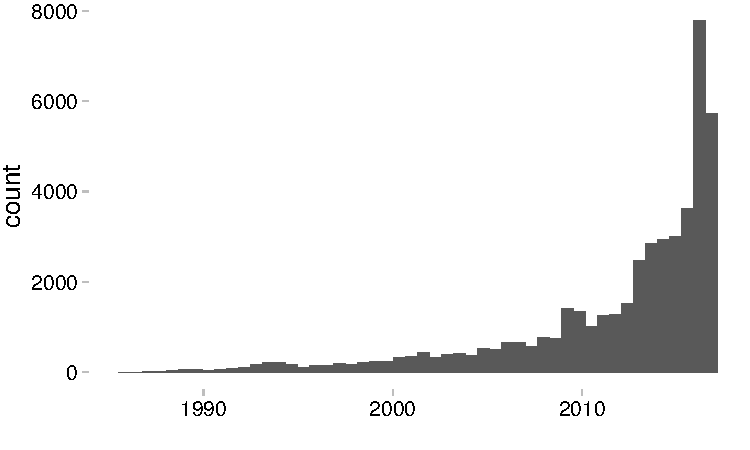
\includegraphics[scale=0.5]{white_paper_files/date_hist}
	\caption{Distribution of Prepayment Samples by Date}
	\label{fig:date_hist}
\end{SCfigure}
\subsection{Factors}
Prepayment models are traditionally broken into \emph{Turnover} and \emph{Refinance} components, where "turnover" means prepayments due to property sales, and "refinancing" means prepayments due to refinancing. With the model structure we used, there is no practical impact to making this division. Some factors arguably belong in both groups, in any case. For example, rises in home prices can propel both house sales and refinancing decisions, as borrowers choose to take equity out of appreciated homes, or take advantage of higher valuations to decrease their loan-to-value ratio, and thus receive better terms on a new loan. 
There is a balance to be struck between the parsimony of a model and its completeness. In the case of GNM pools, there is so much data available that over-identification is unlikely. Building on work done at JPMorgan\cite{jpm_model}, Nikko chose to use a six-factor model, but with some added structural complications, on which more will be discussed in subsection~\ref{subsec:model}. The factors are as follows:
\begin{itemize}
	\item \emph{Incentive}:	The difference between the mortgage coupon and the current prevailing mortgage rate. This is the borrower's incentive to refinance.
	\item \emph{Upfront MIP}: Upfront mortgage insurance payment as a percentage. Borrowers with a large upfront payment may have credit constraints that prevent them from refinancing.
	\item \emph{Home Price Appreciation} (HPA): The amount by which homes in the area have appreciated. GNM provides US Census Metropolitan Statistical Area (MSA) codes, and percentages showing how much of the pool relates to each code. Where possible, we matched the top three MSA codes to S\&P CoreLogic Case-Shiller Home Price indexes, and weighted appropriately. Where loans were mostly outside major metropolitan areas, we used the CoreLogic Median Existing Home Price indexes by State.
	\item \emph{Curve at Origination} (CATO): The difference in spreads between the long end and the short end of the yield curve between the current date and the origination date. I.e. $(10Y_t - 2Y_t) - (10Y_0 - 2Y_0)$. This is meant to show any additional urgency in the borrower's decision to refinance at a given moment.
	\item \emph{Spread at Origination} (SATO): The spread between the weighted average coupon of the pool and the prevailing mortgage rate at origination. A high SATO would suggest potential credit problems, and thus possible difficulties in sourcing a new loan.
	\item \emph{Burnout}: The cumulative prior incentive. I.e. the sum of the difference between the current mortgage coupon and contemporary prevailing mortgage rates in past months. These are the incentives to prepay that the borrower passed up, and may indicate circumstances that make the borrower less likely to refinance or sell his property in the future.
\end{itemize}

\subsection{Model}
\label{subsec:model}
The past three decades have seen explosive growth in the attention paid to probabilistic, i.e. Bayesian, modeling. As computers have grown more powerful, problems that in the past would have been simplified and solved analytically can now be modeled directly using Monte Carlo (MCMC) techniques. We elected to use the software package Stan\cite{stan}, which permits fast prototyping of generative probabilistic models, using Hamiltonian Monte Carlo, which is an advance on the older technique of Markov Chain Monte Carlo with Gibbs Sampling\cite{betancourt2017conceptual}. Stan is at the forefront of modern machine learning research. Astrophysicists have used Stan to analyze gravitational waves\cite{abbott2016rate}. Facebook has recently released a software package, Prophet, that builds on Stan to predict time series with multiple levels of periodicity.

\begin{SCfigure}
	\centering
	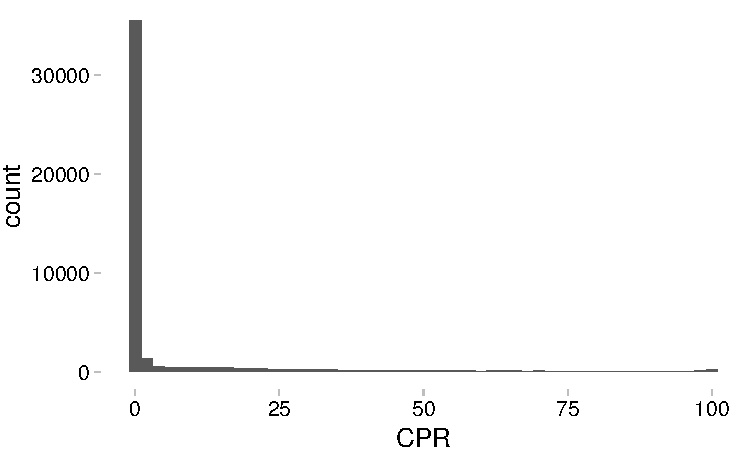
\includegraphics[scale=0.5]{white_paper_files/cpr_hist}
	\caption{Distribution of Monthly CPRs. About 70\% of all months have no prepayment.}
	\label{fig:cpr_hist}
\end{SCfigure}
We elected to model the next-month Conditional Prepayment Rate (CPR) directly as a Poisson distribution. Work has been done using a proportional hazards model to predict actual payments on mortgage pools\cite{popova2008bayesian},  but we feel the preponderance of zero values in the CPR data makes the Beta distribution a Bayesian proportional hazards model uses a poor fit. Additionally, it is not clear from Popova's paper how she and her colleagues account for the large variation in mortgage pool sizes when modeling actual payments. In order to account for the fact that a prepayment is a rare event in any given loan~\ref{fig:cpr_hist}, we add a hurdle term, $\theta$, to predict the likelihood of no prepayment, then regress the exponentiated factors mentioned above on the remaining data. The log-likelihood function is defined by 
%
\[
p(y|\theta,\lambda)
= 
\begin{cases}
\ \theta & \mbox{if } y = 0, \mbox{ and}
\\
\ (1 - \theta)
  \
   \frac{\displaystyle \distro{Poisson}(y | \lambda)}
        {\displaystyle \vspace*{8pt} 1 - \distro{PoissonCDF}(0 | \lambda)}
& \mbox{if } y > 0,
\end{cases}
\]
%
where $\distro{PoissonCDF}$ is the cumulative distribution function for the Poisson distribution\cite{stan_manual}, and $\lambda$ is the exponent of the sum of factor effects.

\begin{figure}
	\centering
	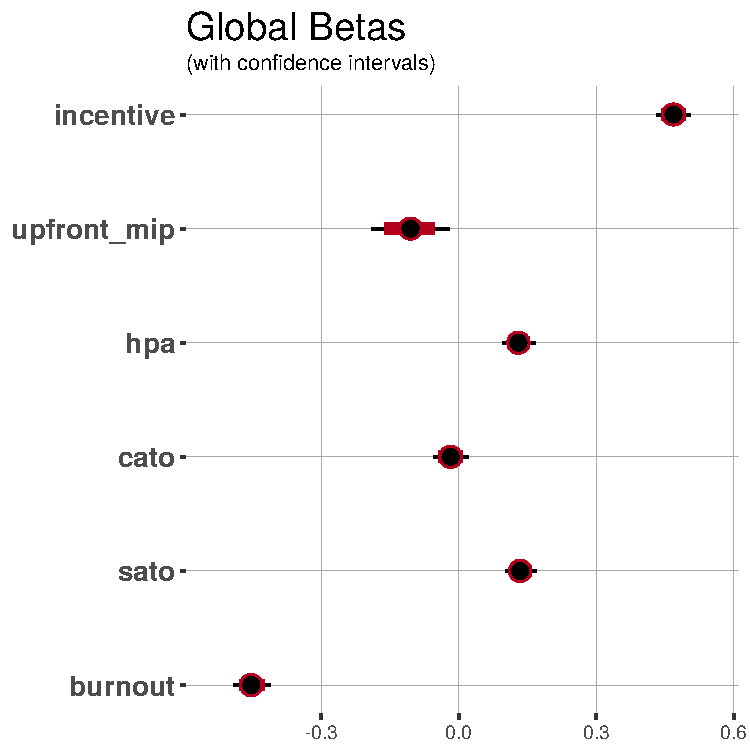
\includegraphics[scale=0.5]{white_paper_files/global_betas}
	\caption{Global betas with confidence intervals}
	\label{fig:global_beta}
\end{figure}
Next, to account for the evolution of underwriting standards and of the available pool of borrowers in general, we fit a multi-level hiearchical model, extracting overall factor betas while permitting varied effects for each pool origination year. The global betas show high confidence in all values except upfront\_mip, which is possibly the result of the dearth of upfront\_mip data for ealier pools (figure~\ref{fig:global_beta}). The per-year betas show strong serial correlation, which is comforting in that it suggests they are not over-fit. It is also possible to see the recovery of the sales market a few years after the credit crisis in the per-year burnout betas (figure ~\ref{fig:vintage_beta}).

\begin{figure}
	\centering
	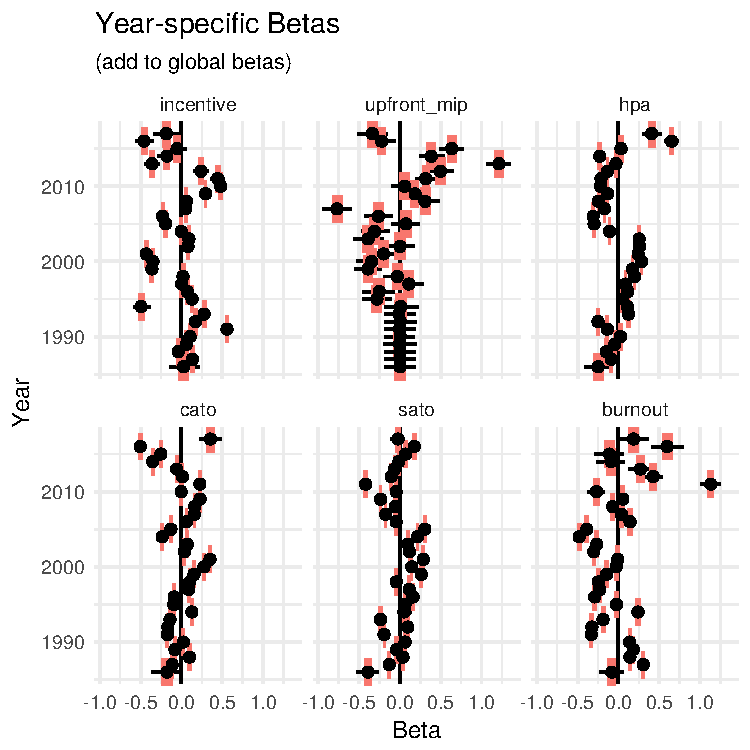
\includegraphics[scale=1]{white_paper_files/vintage_betas}
	\caption{Betas by Pool Origination Year. These should be added to the global betas (figure~\ref{fig:global_beta}), and so represent deviations from the mean}
	\label{fig:vintage_beta}
\end{figure}
\section{Further Work}
Mortgage Pool Prepayments are a challenge to model, and we believe there is much room for improvement in the framework outlined above. It may be advisable to add an additional hierarchy on pool originators, as we currently assume that each firm applies the same standards in bundling loans. We also would like to find better data for early pool years in order to flesh out our model for a rising interest rate environment. Ginnie Mae provides loan-level data in addition to the pool-level data we used here, and we believe we should be able to use that to complement or even replace the current pool-level data. Finally, we believe there may be some value in fitting a mixed effects proportional hazards model.
\newpage
\printbibliography
\end{document}
